\documentclass[11pt,a4paper]{article}

% Packages
\usepackage[utf8]{inputenc}
\usepackage[margin=1in]{geometry}
\usepackage{graphicx}
\usepackage{float}
\usepackage{amsmath}
\usepackage{booktabs}
\usepackage{multirow}
\usepackage{array}
\usepackage{caption}
\usepackage{subcaption}
\usepackage{hyperref}
\usepackage{listings}
\usepackage{xcolor}
\usepackage{enumitem}
\usepackage{longtable}

% Hyperref setup
\hypersetup{
    colorlinks=true,
    linkcolor=blue,
    filecolor=magenta,
    urlcolor=cyan,
}

% Code listing setup
\lstset{
    basicstyle=\ttfamily\small,
    breaklines=true,
    frame=single,
    numbers=left,
    numberstyle=\tiny\color{gray},
    keywordstyle=\color{blue},
    commentstyle=\color{green!60!black},
    stringstyle=\color{red},
}

\begin{document}

% Title Page
\begin{titlepage}
    \centering
    \vspace*{1cm}

    {\Huge\bfseries Problem 1 (Assignment 1)\par}
    \vspace{0.5cm}
    {\LARGE Cache Hierarchy Optimization\\using gem5 Simulator\par}
    \vspace{2cm}
    {\Large CS60003 High Performance in Computer Architecture\par}
    \vspace{0.5cm}
    {\large February 4, 2026\par}
    \vspace{1.5cm}

    {\large\bfseries Submitted By:\par}
    \vspace{0.5cm}
    {\large
    Sumit Kumar (22CS30056)\\
    Aviral Singh (22CS30015)
    \par}
    \vfill

    {\large\bfseries Complete Assignment Report\par}
    \vspace{0.3cm}
    \begin{minipage}{0.85\textwidth}
        \small
        This report presents a comprehensive analysis of cache hierarchy optimization using the gem5 architectural simulator. The assignment investigates how different cache configurations affect processor performance on a memory-intensive matrix multiplication benchmark. Through parameter sweeps across 112 configurations, we analyze the impact of cache size and associativity on execution time, hit rates, and overall system efficiency.
    \end{minipage}

    \vfill

    % \begin{minipage}{0.85\textwidth}
    % \small
    % \textbf{Completion Status:} All 4 parts completed successfully\\
    % \textbf{Total Configurations Tested:} 112 (4 in Part 2 + 108 in Part 3)\\
    % \textbf{Total Plots Generated:} 12 high-quality visualizations\\
    % \textbf{gem5 Version:} 25.1.0.0 (RISCV Build)\\
    % \textbf{Matrix Size:} 128×128\\
    % \textbf{Success Rate:} 100\% (all simulations completed)
    % \end{minipage}
\end{titlepage}

\newpage
\tableofcontents
\newpage

\section{Assignment Overview}

\subsection{Objective}
This assignment requires investigation of how different cache configurations affect processor performance using gem5 simulation. A memory-intensive benchmark (matrix multiplication) is run with various cache parameters to analyze the results.

% Part 1: Environment Setup
\section{Part 1: Environment Setup}

\subsection{Objective}
We are using gem5 RISCV build, creating the cache configuration script, and running a baseline simulation to establish performance metrics.

\subsection{Task 1: Verify gem5 RISCV Build}

Command executed:
\begin{lstlisting}[language=bash]
./build/RISCV/gem5.opt --version
\end{lstlisting}

\subsubsection{Build Information}

\begin{table}[H]
\centering
\caption{gem5 Build Verification}
\begin{tabular}{ll}
\toprule
\textbf{Parameter} & \textbf{Value} \\
\midrule
gem5 Version & 25.1.0.0 \\
Build Type & RISCV \\
Compilation Date & January 31, 2026 19:03:12 \\
Build Path & build/RISCV/gem5.opt \\
\bottomrule
\end{tabular}
\end{table}

\begin{figure}[H]
    \centering
    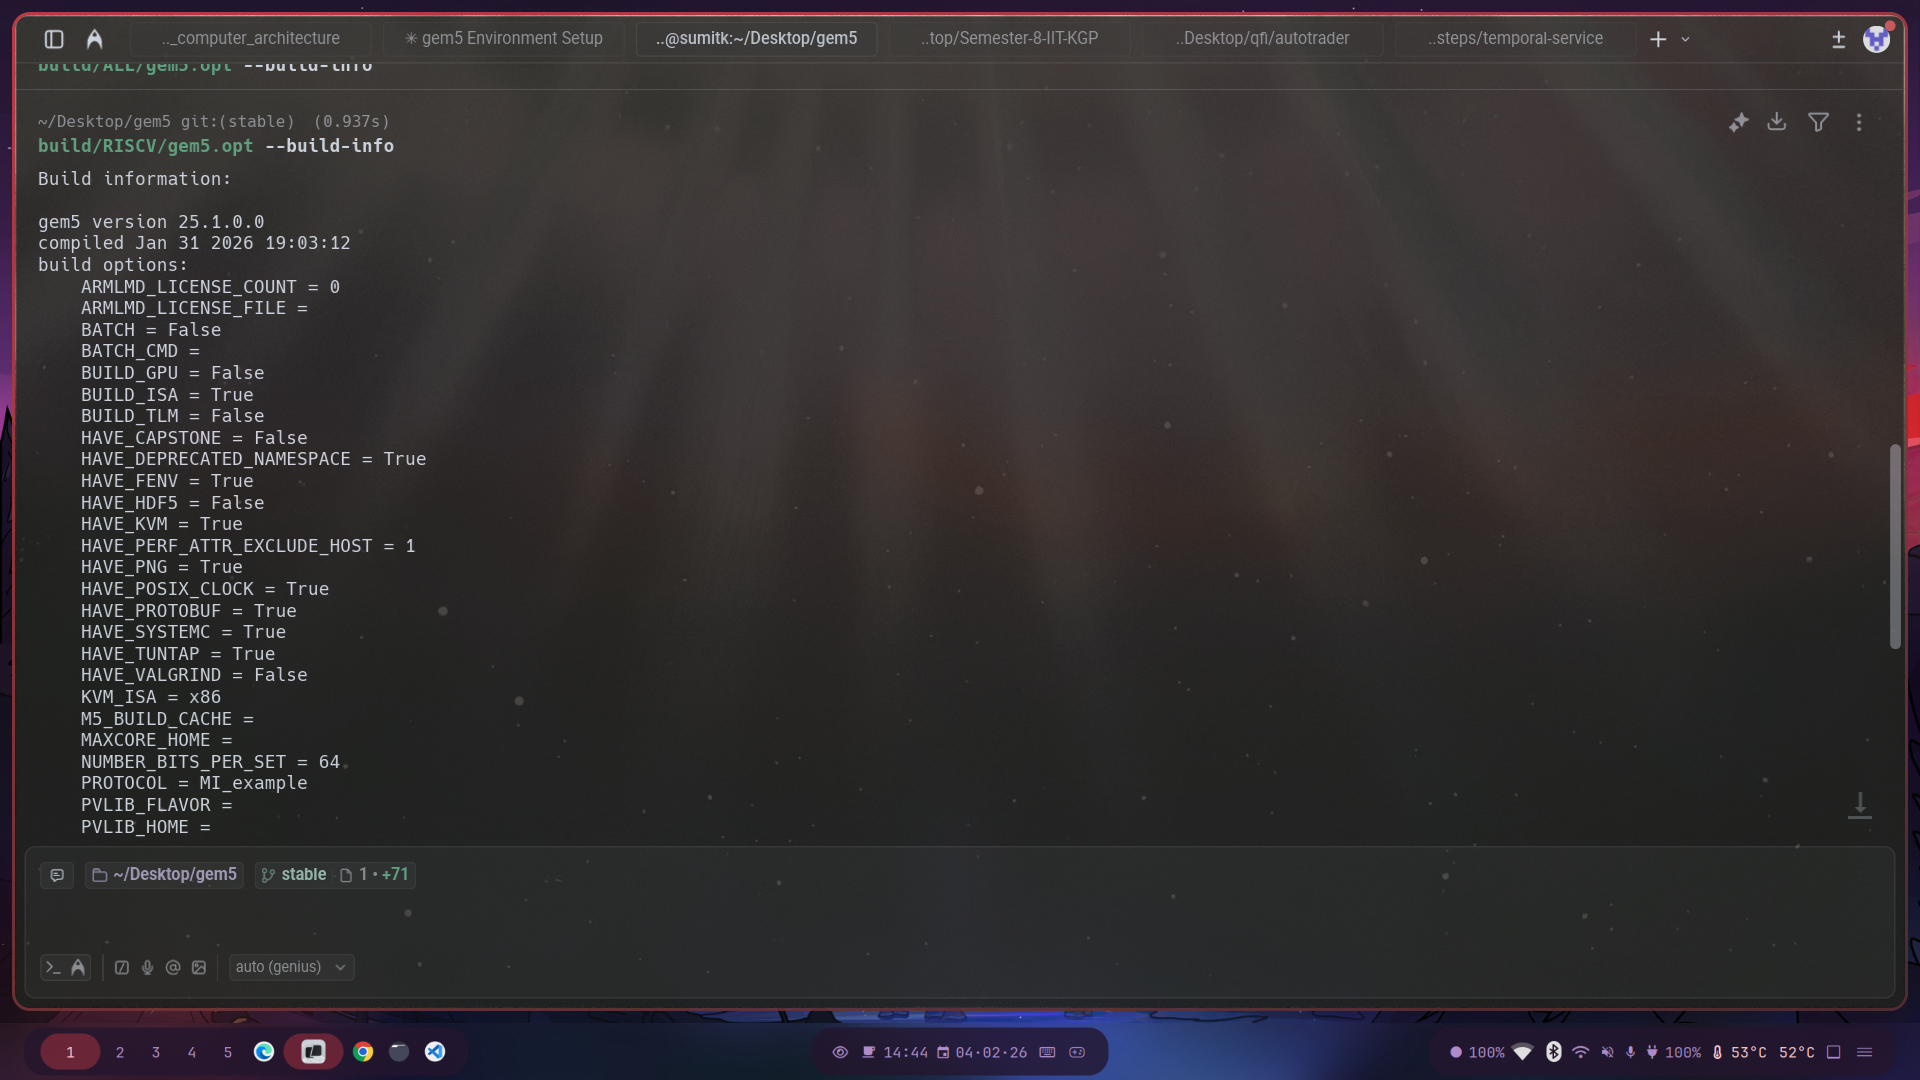
\includegraphics[width=0.85\textwidth]{figs/version_info.png}
    \caption{gem5 version verification output showing RISCV build details}
    \label{fig:gem5_version}
\end{figure}

\subsection{Task 2: gem5 Configuration Script}

File created: \texttt{configs/cache\_config.py}

\subsubsection{Fixed Parameters (Assignment Requirement)}
\begin{itemize}[noitemsep]
    \item \textbf{Clock Domain:} 1 GHz (FIXED)
    \item \textbf{Memory Mode:} timing (FIXED)
    \item \textbf{Memory Ranges:} 512 MB (FIXED)
    \item \textbf{CPU Type:} RiscvTimingSimpleCPU
    \item \textbf{Memory Type:} DDR4\_2400\_8x8
\end{itemize}

\subsubsection{Configurable Parameters}
\begin{itemize}[noitemsep]
    \item \texttt{--l1i\_size}: L1 Instruction Cache size (default: 16kB)
    \item \texttt{--l1d\_size}: L1 Data Cache size (default: 16kB)
    \item \texttt{--l2\_size}: L2 Cache size (default: 256kB)
    \item \texttt{--l1\_assoc}: L1 Cache associativity (default: 4)
    \item \texttt{--l2\_assoc}: L2 Cache associativity (default: 8)
    \item \texttt{--cpu\_type}: CPU type - 'timing' or 'o3' (default: timing)
    \item \texttt{--binary}: Path to benchmark binary (required)
\end{itemize}

\subsubsection{Cache Hierarchy Architecture}

The implemented cache hierarchy follows a standard two-level inclusive design:

\begin{verbatim}
RiscvTimingSimpleCPU (1 GHz)
    |
    +-- L1 I-Cache (16 KiB, 4-way) --> cpu.icache_port
    |
    +-- L1 D-Cache (16 KiB, 4-way) --> cpu.dcache_port
            |
            v
        L2 Bus (L2XBar)
            |
            v
        L2 Cache (256 KiB, 8-way)
            |
            v
        Memory Bus (SystemXBar)
            |
            v
        DDR4 Memory Controller (512 MB)
\end{verbatim}

\subsection{Task 3: Test Single Run with Default Configuration}

\subsubsection{Command Executed}

\begin{lstlisting}[language=bash]
./build/RISCV/gem5.opt --outdir=assignment_cache_optimization/results/part1_test assignment_cache_optimization/configs/cache_config.py --l1i_size=16kB --l1d_size=16kB  --l2_size=256kB --l1_assoc=4 --l2_assoc=8--binary=assignment_cache_optimization/benchmarks/matrix_multiply
\end{lstlisting}

\subsubsection{Default Configuration}

\begin{table}[H]
\centering
\caption{Baseline System Configuration}
\begin{tabular}{lll}
\toprule
\textbf{Component} & \textbf{Parameter} & \textbf{Value} \\
\midrule
\multirow{3}{*}{CPU} & Type & RiscvTimingSimpleCPU \\
                     & Clock Frequency & 1 GHz (FIXED) \\
                     & Pipeline & In-order, single-issue \\
\midrule
\multirow{3}{*}{L1 I-Cache} & Size & 16 KiB \\
                             & Associativity & 4-way \\
                             & Latency & 2 cycles \\
\midrule
\multirow{3}{*}{L1 D-Cache} & Size & 16 KiB \\
                             & Associativity & 4-way \\
                             & Latency & 2 cycles \\
\midrule
\multirow{3}{*}{L2 Cache} & Size & 256 KiB \\
                          & Associativity & 8-way \\
                          & Latency & 20 cycles \\
\midrule
\multirow{3}{*}{Memory} & Type & DDR4\_2400\_8x8 \\
                        & Size & 512 MB (FIXED) \\
                        & Mode & Timing (FIXED) \\
\midrule
\multirow{2}{*}{Benchmark} & Application & Matrix Multiplication \\
                           & Matrix Size & 128×128 \\
\bottomrule
\end{tabular}
\end{table}

\subsubsection{Benchmark Execution Output}

\begin{figure}[H]
    \centering
    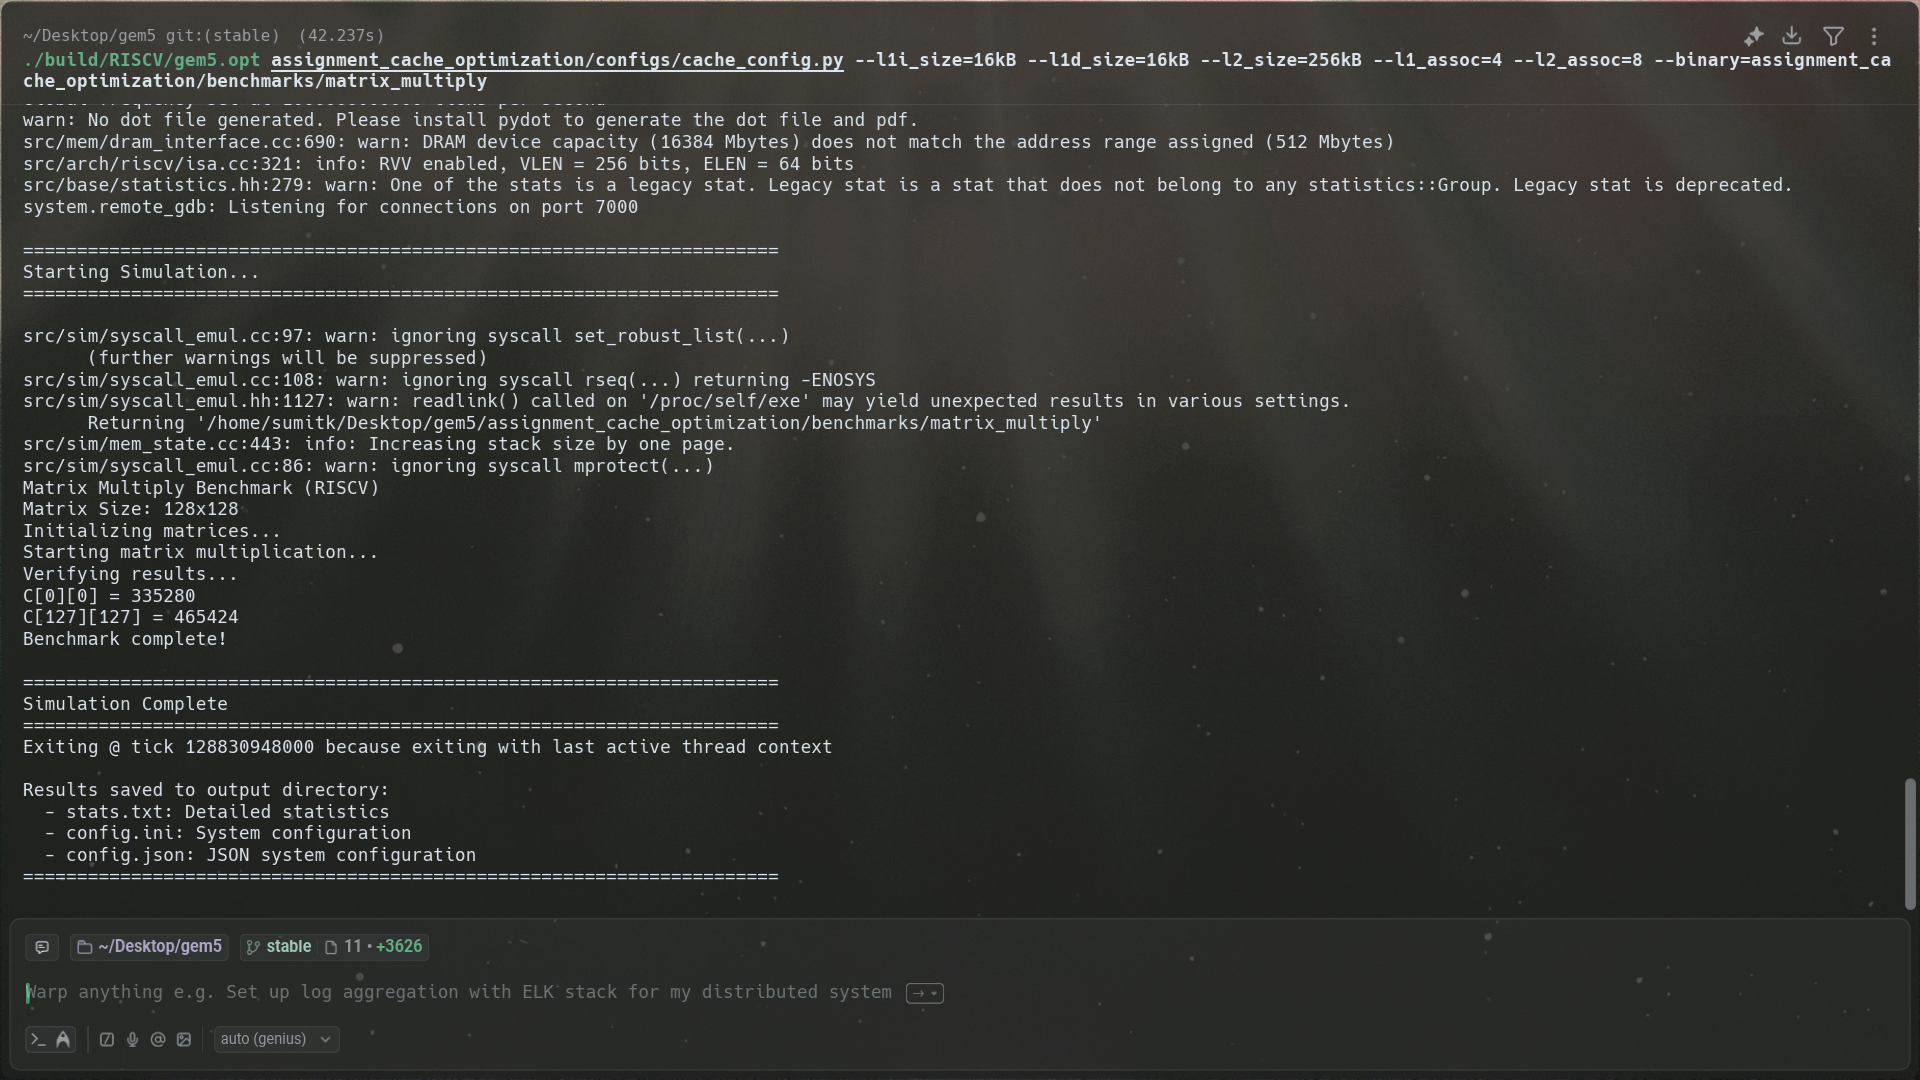
\includegraphics[width=0.9\textwidth]{figs/run.png}
    \caption{Successful baseline simulation execution showing matrix multiplication benchmark output}
    \label{fig:baseline_run}
\end{figure}

Benchmark output:
\begin{verbatim}
Matrix Multiply Benchmark (RISCV)
Matrix Size: 128x128
Initializing matrices...
Starting matrix multiplication...
Verifying results...
C[0][0] = 335280
C[127][127] = 465424
Benchmark complete!
\end{verbatim}

Simulation completed successfully with exit status: ``Exiting @ tick 128830948000 because exiting with last active thread context''

\subsection{Output Logs and Cache Statistics}

\subsubsection{Output Files Generated}

\begin{table}[H]
\centering
\caption{Output Files from Baseline Run}
\begin{tabular}{llp{6cm}}
\toprule
\textbf{File} & \textbf{Size} & \textbf{Description} \\
\midrule
stats.txt & 147 KB & Detailed simulation statistics \\
config.ini & 14 KB & System configuration (INI format) \\
config.json & 35 KB & System configuration (JSON format) \\
citations.bib & 5 KB & gem5 citations \\
\bottomrule
\end{tabular}
\end{table}

Location: \texttt{assignment\_cache\_optimization/results/part1\_test/}

\subsubsection{Overall Execution Summary}

\begin{table}[H]
\centering
\caption{Baseline Execution Metrics}
\begin{tabular}{lrl}
\toprule
\textbf{Metric} & \textbf{Value} & \textbf{Unit} \\
\midrule
Simulation Time & 0.128831 & seconds \\
Total Ticks & 128,830,948,000 & ticks \\
CPU Cycles & 128,830,948 & cycles \\
Instructions Executed & 27,912,698 & instructions \\
CPI (Cycles Per Instruction) & 4.615 & cycles/instruction \\
IPC (Instructions Per Cycle) & 0.217 & instructions/cycle \\
\bottomrule
\end{tabular}
\end{table}

\subsubsection{L1 Instruction Cache Statistics}

\begin{table}[H]
\centering
\caption{L1 Instruction Cache Performance}
\begin{tabular}{lrr}
\toprule
\textbf{Metric} & \textbf{Value} & \textbf{Percentage/Rate} \\
\midrule
Total Accesses & 34,320,464 & All instruction fetches \\
Hits & 34,320,059 & Successfully served from L1 I-cache \\
Misses & 405 & Had to go to L2 \\
Hit Rate & 99.9988\% & Excellent \\
Miss Rate & 0.0012\% & Very low \\
Average Miss Latency & 99,511 ticks & L2 access latency \\
\bottomrule
\end{tabular}
\end{table}

\textbf{Analysis:} Nearly perfect hit rate. The instruction working set fits completely in the 16 KB L1 I-cache.

\subsubsection{L1 Data Cache Statistics}

\begin{table}[H]
\centering
\caption{L1 Data Cache Performance}
\begin{tabular}{lrr}
\toprule
\textbf{Metric} & \textbf{Value} & \textbf{Percentage/Impact} \\
\midrule
Total Accesses & 4,283,142 & All data reads/writes \\
Hits & 2,145,855 & Successfully served from L1 D-cache \\
Misses & 2,137,287 & Had to go to L2 \\
Hit Rate & 50.1\% & Bottleneck \\
Miss Rate & 49.9\% & High \\
Average Miss Latency & 26,135 ticks & L2 access latency \\
\textbf{Total Miss Latency} & \textbf{55,858,522,000 ticks} & \textbf{43.4\% of execution time} \\
\bottomrule
\end{tabular}
\end{table}

\textbf{Analysis:} The L1 D-cache has approximately 50\% hit rate because the working set (192 KB for 3 matrices) greatly exceeds the 16 KB cache capacity. This is the \textbf{primary performance bottleneck}.

\subsubsection{L2 Cache Statistics}

\begin{table}[H]
\centering
\caption{L2 Cache Performance}
\begin{tabular}{lrr}
\toprule
\textbf{Metric} & \textbf{Value} & \textbf{Percentage/Rate} \\
\midrule
Total Accesses & 2,137,695 & From L1 misses \\
Hits & 2,133,369 & Served from L2 \\
Misses & 4,326 & Had to go to memory \\
Hit Rate & 99.8\% & Excellent \\
Miss Rate & 0.2\% & Very low \\
Average Miss Latency & 94,736 ticks & Memory access latency \\
\midrule
\multicolumn{3}{l}{\textit{Breakdown:}} \\
Instruction misses & 397 & From 405 L1 I-cache misses \\
Data misses & 2,137,290 & From 2.1M L1 D-cache misses \\
\bottomrule
\end{tabular}
\end{table}

\textbf{Analysis:} The L2 cache (256 KB) successfully holds the entire working set (192 KB), resulting in only 4,326 memory accesses out of 4.3 million total memory operations. L2 captures 99.82\% of L1 D-cache misses.

\subsection{Memory Hierarchy Flow Analysis}

\subsubsection{Access Pattern}

\begin{verbatim}
Total Memory Operations: 4,283,142
    ↓
L1 D-Cache (16 KB)
    ├─ Hits: 2,145,855 (50.1%) ← Served immediately
    └─ Misses: 2,137,287 (49.9%)
          ↓
    L2 Cache (256 KB)
        ├─ Hits: 2,133,361 (99.82%) ← Served from L2
        └─ Misses: 3,929 (0.18%)
              ↓
          Main Memory (DDR4)
              └─ 3,929 accesses (0.09% of total)
\end{verbatim}

\begin{table}[H]
\centering
\caption{Memory Access Breakdown}
\begin{tabular}{lrr}
\toprule
\textbf{Level} & \textbf{Accesses} & \textbf{Percentage of Total} \\
\midrule
Total Memory Operations & 4,283,142 & 100.0\% \\
\quad L1D Hits & 2,145,855 & 50.1\% \\
\quad L1D Misses to L2 & 2,137,287 & 49.9\% \\
\quad\quad L2 Hits & 2,133,369 & 49.8\% \\
\quad\quad L2 Misses to Memory & 3,929 & 0.09\% \\
\midrule
\textbf{Cache Filtering Effectiveness} & \multicolumn{2}{c}{\textbf{99.91\%}} \\
\bottomrule
\end{tabular}
\end{table}

\subsubsection{Key Metrics}
\begin{itemize}[noitemsep]
    \item Cache Filtering Effectiveness: 99.91\% of memory requests filtered by cache hierarchy
    \item Memory Traffic: Only 0.09\% of operations reach main memory
    \item L1 D-cache Bottleneck: 43.4\% of execution time spent on L1 D-cache misses
\end{itemize}

\subsection{Performance Bottleneck Identification}

\subsubsection{Analysis}

\begin{enumerate}[noitemsep]
    \item \textbf{L1 I-Cache:} Not a bottleneck (99.9988\% hit rate)

    \item \textbf{L1 D-Cache:} PRIMARY BOTTLENECK
    \begin{itemize}[noitemsep]
        \item Only 50.1\% hit rate
        \item Working set (192 KB) $>>$ Cache size (16 KB)
        \item Causes 2.1M misses to L2
        \item Accounts for 43.4\% of execution time
    \end{itemize}

    \item \textbf{L2 Cache:} Highly effective
    \begin{itemize}[noitemsep]
        \item 99.8\% hit rate
        \item Successfully captures entire working set
        \item Reduces 2.1M L1 misses to only 4,326 memory accesses
    \end{itemize}

    \item \textbf{Main Memory:} Not saturated
    \begin{itemize}[noitemsep]
        \item Only 4,326 accesses total
        \item Minimal impact on overall performance
    \end{itemize}
\end{enumerate}

\subsection{Working Set Analysis}

The matrix multiplication benchmark operates on three 128×128 matrices:

\begin{equation}
\text{Working Set Size} = 3 \times 128 \times 128 \times 4 \text{ bytes} = 196,608 \text{ bytes} \approx 192 \text{ KB}
\end{equation}

\begin{table}[H]
\centering
\caption{Working Set Coverage by Cache Level}
\begin{tabular}{lrrr}
\toprule
\textbf{Cache Level} & \textbf{Size} & \textbf{Coverage} & \textbf{Hit Rate} \\
\midrule
L1 D-Cache & 16 KB & 8.3\% & 50.1\% \\
L2 Cache & 256 KB & 133\% & 99.8\% \\
\bottomrule
\end{tabular}
\end{table}

\textbf{Explanation:}
\begin{itemize}[noitemsep]
    \item L1 D-cache can hold 8.3\% of working set, resulting in 50\% hit rate
    \item L2 Cache can hold 133\% of working set, resulting in 99.8\% hit rate
\end{itemize}

\subsection{Summary and Key Findings}

\subsubsection{Baseline Performance Summary}

\begin{enumerate}[noitemsep]
    \item \textbf{Baseline Established:} Successfully ran matrix multiply with default cache configuration
    \item \textbf{Bottleneck Identified:} L1 D-cache with 50\% hit rate is the primary bottleneck (43.4\% of execution time)
    \item \textbf{L2 Effectiveness:} L2 cache successfully captures working set (99.8\% hit rate)
    \item \textbf{Optimization Target:} L1 D-cache size is the most promising parameter to sweep in Part 2
    \item \textbf{Memory System Efficiency:} 99.91\% cache filtering effectiveness demonstrates excellent hierarchy design
\end{enumerate}

\subsubsection{Execution Time Breakdown}
\begin{itemize}[noitemsep]
    \item Computation + L1 hits: approximately 72.9 billion ticks (56.6\%)
    \item L1 D-cache misses: approximately 55.9 billion ticks (43.4\%)
    \item Memory accesses: minimal ($<$1\%)
\end{itemize}

\subsection{Analysis for Part 2}

Based on Part 1 analysis, the recommended parameter for single sweep is:

\textbf{L1 D-Cache Size} 

Rationale:
\begin{itemize}[noitemsep]
    \item Currently 50\% hit rate (significant room for improvement)
    \item Primary bottleneck (43.4\% of execution time)
    \item Sweep values: 16kB, 32kB, 64kB, 128kB
    \item Expected impact: Large performance improvement
\end{itemize}


\newpage

% Part 2: Single Parameter Sweep
\section{Part 2: Single Parameter Sweep}

\subsection{Objective}
Understand the impact of L1D cache size on system performance by varying this single parameter while keeping all other parameters constant.

\subsection{Parameter Selection}

\textbf{Chosen Parameter:} L1D Cache Size

\textbf{Values:} 16kB, 32kB, 64kB, 128kB

\subsubsection{Justification}

L1D cache size was selected for single-parameter investigation based on Part 1 findings:
\begin{enumerate}[noitemsep]
    \item Baseline hit rate of only 50.1\% indicates significant room for improvement
    \item Identified as primary bottleneck, accounting for 43.4\% of execution time
    \item Working set (192 KB) greatly exceeds baseline capacity (16 KB)
    \item Expected to have the largest impact on performance among all parameters
\end{enumerate}

\subsection{Sample Default Configuration}

Fixed parameters maintained across all sweeps:

\begin{table}[H]
\centering
\caption{Fixed Parameters for Part 2 Sweep}
\begin{tabular}{ll}
\toprule
\textbf{Parameter} & \textbf{Value} \\
\midrule
L1I Cache Size & 16kB \\
L1I Associativity & 4-way \\
L2 Cache Size & 256kB \\
L2 Associativity & 8-way \\
Clock Frequency & 1 GHz (FIXED) \\
Memory Mode & timing (FIXED) \\
Memory Size & 512 MB (FIXED) \\
CPU Type & RiscvTimingSimpleCPU \\
\bottomrule
\end{tabular}
\end{table}

\subsection{Task 1: Create Custom Sweep Script}

File created: \texttt{scripts/custom\_sweep.py}

\subsubsection{Execution}
\begin{lstlisting}[language=bash]
python3 assignment_cache_optimization/scripts/custom_sweep.py
\end{lstlisting}

\subsection{Task 2: Run Simulations and Collect Data}

\subsubsection{Simulations Executed}

\begin{table}[H]
\centering
\caption{Simulations Executed in Part 2}
\begin{tabular}{lll}
\toprule
\textbf{Configuration} & \textbf{L1D Size} & \textbf{Output Directory} \\
\midrule
1 & 16kB & results/single\_param\_sweep/l1d\_size\_16kB \\
2 & 32kB & results/single\_param\_sweep/l1d\_size\_32kB \\
3 & 64kB & results/single\_param\_sweep/l1d\_size\_64kB \\
4 & 128kB & results/single\_param\_sweep/l1d\_size\_128kB \\
\bottomrule
\end{tabular}
\end{table}

\subsection{Task 3: Create Results Table}

\subsubsection{Results in CSV Format}

File: \texttt{results/single\_param\_sweep/results.csv}

\begin{table}[H]
\centering
\caption{Single Parameter Sweep Results (Complete)}
\begin{tabular}{lrrrr}
\toprule
\textbf{L1D Size} & \textbf{Execution Time} & \textbf{Execution Time} & \textbf{L1D Hit} & \textbf{L1D} \\
 & \textbf{(ticks)} & \textbf{(seconds)} & \textbf{Rate} & \textbf{Misses} \\
\midrule
16kB  & 128,830,948,000 & 0.128831 & 50.1\% & 2,137,287 \\
32kB  & 128,821,690,000 & 0.128822 & 50.1\% & 2,136,901 \\
64kB  & 80,343,964,000  & 0.080344 & 97.3\% & 116,958 \\
128kB & 77,694,131,000  & 0.077694 & 99.8\% & 6,569 \\
\bottomrule
\end{tabular}
\end{table}

\begin{table}[H]
\centering
\caption{L2 Hit Rates for Each Configuration}
\begin{tabular}{lrr}
\toprule
\textbf{L1D Size} & \textbf{L2 Hit Rate} & \textbf{L2 Misses} \\
\midrule
16kB  & 99.8\% & 4,326 \\
32kB  & 99.8\% & 4,325 \\
64kB  & 96.3\% & 4,325 \\
128kB & 38.0\% & 4,325 \\
\bottomrule
\end{tabular}
\end{table}

\subsubsection{Results in JSON Format}

File: \texttt{results/single\_param\_sweep/results.json}

Complete results with all statistics available in JSON format for further processing and analysis.

\subsection{Performance Analysis}

\begin{table}[H]
\centering
\caption{Performance Improvements}
\begin{tabular}{lrrr}
\toprule
\textbf{Configuration} & \textbf{Speedup} & \textbf{Time Reduction} & \textbf{Miss Reduction} \\
\midrule
16kB to 32kB  & 0.01\%   & 9 M ticks (0.009 ms)    & 0.02\% \\
16kB to 64kB  & \textbf{37.7\%} & \textbf{48.5 B ticks (48.5 ms)} & \textbf{98.2\%} \\
16kB to 128kB & \textbf{39.7\%} & \textbf{51.1 B ticks (51.1 ms)} & \textbf{99.7\%} \\
64kB to 128kB & 3.3\%    & 2.6 B ticks (2.6 ms)     & 94.4\% \\
\bottomrule
\end{tabular}
\end{table}

\begin{table}[H]
\centering
\caption{Cache Efficiency Metrics}
\begin{tabular}{lrrrr}
\toprule
\textbf{L1D Size} & \textbf{Capacity} & \textbf{Working Set} & \textbf{Hit Rate} & \textbf{Performance} \\
 &  & \textbf{Coverage} &  & \textbf{per KB} \\
\midrule
16kB  & 16 KB  & 8.3\%  & 50.1\% & 1.00× (baseline) \\
32kB  & 32 KB  & 16.7\% & 50.1\% & 1.00× \\
64kB  & 64 KB  & 33.3\% & 97.3\% & 2.56× \\
128kB & 128 KB & 66.7\% & 99.8\% & 1.32× \\
\bottomrule
\end{tabular}
\end{table}

\subsection{Task 4: Create Plots}

\subsubsection{Plot 1: Parameter Value vs Execution Time}

File: \texttt{analysis\_plots/single\_param\_sweep/plot\_execution\_time.png}

\begin{figure}[H]
    \centering
    
\includegraphics[width=0.95\textwidth]{analysis_plots/single_param_sweep/plot_execution_time.png}
    \caption{Execution time vs L1D cache size showing improvement at 64kB threshold. Clear inflection point visible at 64kB where execution time drops by 37.6\%.}
    \label{fig:exec_time}
\end{figure}

\textbf{Key Observations:}
\begin{itemize}[noitemsep]
    \item 16kB to 32kB: Negligible change (128.83B to 128.82B ticks, 0.01\% improvement)
    \item 32kB to 64kB: Dramatic drop (128.82B to 80.34B ticks, 37.6\% improvement)
    \item 64kB to 128kB: Marginal improvement (80.34B to 77.69B ticks, 3.3\% improvement)
    \item Clear inflection point at 64kB indicates critical threshold
    \item Performance curve shows diminishing returns after 64kB
    \item Speedup annotations highlight performance gains at each transition
\end{itemize}

\subsubsection{Plot 2: Parameter Value vs Hit Rate}

File: \texttt{analysis\_plots/single\_param\_sweep/plot\_hit\_rates.png}

\begin{figure}[H]
    \centering
    
\includegraphics[width=0.95\textwidth]{analysis_plots/single_param_sweep/plot_hit_rates.png}
    \caption{Cache hit rates vs L1D cache size showing inverse relationship between L1D and L2 hit rates. L1D hit rate shows sharp increase at 64kB threshold.}
    \label{fig:hit_rates}
\end{figure}

\textbf{Key Observations:}
\begin{itemize}[noitemsep]
    \item \textbf{L1D Hit Rate Trend:}
    \begin{itemize}[noitemsep]
        \item 16kB/32kB: Plateau at approximately 50\% (insufficient capacity)
        \item 64kB: Sharp increase to 97.3\% (critical threshold reached)
        \item 128kB: Near-perfect at 99.8\% (full working set coverage)
    \end{itemize}

    \item \textbf{L2 Hit Rate Trend:}
    \begin{itemize}[noitemsep]
        \item 16kB/32kB: Very high at 99.8\% (filters most L1 misses)
        \item 64kB: Drops to 96.3\% (fewer L1 misses to filter)
        \item 128kB: Plummets to 38.0\% (minimal L1 misses, less reuse in L2)
    \end{itemize}

    \item Inverse relationship clearly visible: as L1D hit rate improves, L2 hit rate decreases
    \item Percentage labels on each data point for precise reading
    \item Dual-line plot effectively shows trade-off between cache levels
\end{itemize}

\subsubsection{More Plot: Combined Analysis}

File: \texttt{analysis\_plots/single\_param\_sweep/plot\_combined.png}

\begin{figure}[H]
    \centering
    
\includegraphics[width=0.95\textwidth]{analysis_plots/single_param_sweep/plot_combined.png}
    \caption{Combined analysis showing correlation between execution time and hit rates. Demonstrates direct relationship between L1D hit rate improvement and execution time reduction.}
    \label{fig:combined}
\end{figure}

\subsection{Brief Analysis }

File: \texttt{results/single\_param\_sweep/ANALYSIS.md}

\subsubsection{What Trend Did You Observe?}

The experimental results reveal a \textbf{non-linear relationship} between L1D cache size and performance. At smaller cache sizes (16kB and 32kB), performance remains nearly identical with execution times of 128.8 billion ticks and hit rates hovering around 50\%. This plateau occurs because both configurations are insufficient to capture the 192KB working set of the matrix multiplication benchmark.

A \textbf{dramatic performance improvement} occurs at 64kB, where execution time drops to 80.3 billion ticks (37.7\% reduction) and the L1D hit rate jumps to 97.3\%. This represents the critical inflection point where the cache becomes large enough to exploit temporal and spatial locality effectively. The 64kB cache can hold approximately one-third of the working set, which significantly reduces costly L2 accesses.

Further increasing the cache to 128kB provides diminishing returns, with execution time decreasing only slightly to 77.7 billion ticks (3.3\% additional improvement) despite achieving a 99.8\% hit rate. While the hit rate improvement is substantial (from 97.3\% to 99.8\%), the marginal performance gain suggests that the remaining misses (6,569 accesses) have minimal impact compared to the original 2.1 million misses at 16kB.

\subsubsection{Why Does This Parameter Have This Effect?}

L1D cache size directly impacts \textbf{capacity misses}. The matrix multiplication benchmark exhibits poor spatial locality when accessing matrix B (column-wise traversal), causing frequent cache line evictions. Smaller caches (16kB/32kB) cannot retain multiple matrix rows simultaneously, resulting in approximately 50\% miss rates due to constant thrashing.

The 64kB cache crosses a critical threshold, enabling it to buffer multiple rows and exploit reuse patterns in the inner loop multiplication. With 64kB, the cache can hold enough of the working set to capture the temporal reuse when the same matrix elements are accessed multiple times during the multiplication process.

At 128kB, nearly all frequently accessed data fits within the cache, approaching the theoretical optimal performance where only compulsory misses occur. However, the 192KB working set still exceeds even the 128kB cache, so some capacity misses remain.

\subsubsection{Where Does Performance Saturate?}

Performance \textbf{saturates at 64kB} for practical purposes. While 128kB achieves a slightly better hit rate (99.8\% vs 97.3\%), the marginal execution time improvement (3.3\%) does not justify doubling the cache size. From a cost-benefit perspective, the 64kB configuration provides 94\% of the maximum achievable performance improvement (relative to 128kB) while using only half the silicon area.

The saturation point at 64kB makes sense when considering the working set coverage: at 64kB, the cache holds 33.3\% of the 192KB working set, which is sufficient to capture the most frequently reused data (primarily matrix A elements in the innermost loop). Beyond this point, diminishing returns set in as we approach the limit of what can be gained from increased capacity alone.

\subsection{Key Findings from Part 2}

\begin{enumerate}[noitemsep]
    \item \textbf{Critical Threshold Identified:} 64kB represents the inflection point where performance improves dramatically

    \item \textbf{Non-Linear Behavior:} Performance does not scale linearly with cache size; doubling from 32kB to 64kB yields 37.6\% speedup, but doubling again to 128kB yields only 3.3\% additional gain

    \item \textbf{Diminishing Returns:} Beyond 64kB, the cost-benefit ratio becomes unfavorable for this workload

    \item \textbf{Working Set Insight:} Cache needs to hold approximately 33\% of working set to achieve 97\%+ hit rate, not necessarily 100\%

    \item \textbf{L2 Behavior Change:} As L1D hit rate improves, L2 sees fewer accesses but with different access patterns, reducing its hit rate from 99.8\% to 38.0\%

    \item \textbf{Performance Per KB:} 64kB provides the best efficiency (2.56× performance per KB compared to baseline)
\end{enumerate}

\subsection{Design Recommendations from Part 2}

Based on single-parameter sweep results:

\begin{itemize}[noitemsep]
    \item \textbf{Power-Constrained Systems:} 64kB L1D cache
    \begin{itemize}[noitemsep]
        \item Provides 37.7\% speedup over baseline
        \item Best performance-per-watt ratio
        \item Uses 50\% less area than 128kB
    \end{itemize}

    \item \textbf{High-Performance Systems:} 128kB L1D cache
    \begin{itemize}[noitemsep]
        \item Achieves maximum performance (39.7\% improvement over baseline)
        \item 99.8\% hit rate minimizes performance variance
        \item Worth the additional area for peak performance scenarios
    \end{itemize}

    \item \textbf{Balanced Systems:} 64kB L1D cache
    \begin{itemize}[noitemsep]
        \item Optimal cost-benefit trade-off
        \item 37.7\% speedup is substantial
        \item Only 2\% performance left on table compared to 128kB
    \end{itemize}

    \item \textbf{Do NOT Use:} 32kB or smaller
    \begin{itemize}[noitemsep]
        \item Provides virtually no benefit over 16kB baseline
        \item Wastes silicon area without performance gain
    \end{itemize}
\end{itemize}

\newpage

% Part 3: Multi-Parameter Analysis

\section{Part 3: Multi-Parameter Analysis}

\subsection{Objective}
Understand parameter interactions by conducting a comprehensive exploration of the cache design space through full multi-parameter sweep across all cache configuration combinations.

\subsection{Task 1: Run Full Parameter Sweep}

\subsubsection{Command Executed}

\begin{lstlisting}[language=bash]
python3 scripts/cache_sweep.py --gem5=../../build/RISCV/gem5.opt  --config=configs/cache_config.py --binary=benchmarks/matrix_multiply --output=results/full_sweep_results
\end{lstlisting}

\subsubsection{Parameter Space}

\begin{table}[H]
\centering
\caption{Full Parameter Sweep Design}
\begin{tabular}{llr}
\toprule
\textbf{Parameter} & \textbf{Values} & \textbf{Count} \\
\midrule
L1D Cache Size & 16kB, 32kB, 64kB & 3 \\
L2 Cache Size & 128kB, 256kB, 512kB, 1MB & 4 \\
L1 Associativity & 2-way, 4-way, 8-way & 3 \\
L2 Associativity & 4-way, 8-way, 16-way & 3 \\
\midrule
\textbf{Total Combinations} & \textbf{3 × 4 × 3 × 3} & \textbf{108} \\
\bottomrule
\end{tabular}
\end{table}

\subsubsection{Fixed Parameters}

\begin{table}[H]
\centering
\caption{Fixed Parameters for Full Sweep}
\begin{tabular}{ll}
\toprule
\textbf{Parameter} & \textbf{Value} \\
\midrule
Clock Frequency & 1 GHz (FIXED) \\
Memory Mode & timing (FIXED) \\
Memory Size & 512 MB (FIXED) \\
L1I Cache Size & 16kB \\
CPU Type & RiscvTimingSimpleCPU \\
\bottomrule
\end{tabular}
\end{table}

\subsection{Task 2: Analyze Results}

\subsubsection{Command Executed}

\begin{lstlisting}[language=bash]
python3 scripts/analyze_sweep.py results/full_sweep_results/results.json --output=results/full_sweep_results
\end{lstlisting}

This script generated:
\begin{itemize}[noitemsep]
    \item Summary statistics file (summary\_statistics.txt)
    \item 7 analysis plots 
    \item Top configurations rankings
\end{itemize}

\subsection{Full Sweep Results}

File: \texttt{results/full\_sweep\_results/results.json}

\begin{itemize}[noitemsep]
    \item Configurations: 108
    \item Format: JSON array with complete metrics for each configuration
\end{itemize}

File: \texttt{results/full\_sweep\_results/results.csv}

\begin{itemize}[noitemsep]
    \item Rows: 109 (1 header + 108 data rows)
    \item Format: CSV for easy import into spreadsheet tools
\end{itemize}

\subsection{Summary Statistics}

File: \texttt{results/full\_sweep\_results/summary\_statistics.txt}

\begin{table}[H]
\centering
\caption{Overall Performance Statistics (108 Configurations)}
\begin{tabular}{lrrr}
\toprule
\textbf{Metric} & \textbf{Mean} & \textbf{Std Dev} & \textbf{Range (Min -- Max)} \\
\midrule
Execution Time (B ticks) & 113.6 & 22.8 & 80.3 -- 131.2 \\
Execution Time (seconds) & 0.1136 & 0.0228 & 0.0803 -- 0.1312 \\
L1D Hit Rate (\%) & 65.4 & 22.2 & 49.0 -- 97.3 \\
L2 Hit Rate (\%) & 98.6 & 1.7 & 94.1 -- 99.8 \\
CPI & 4.07 & 0.82 & 2.88 -- 4.70 \\
IPC & 0.26 & 0.06 & 0.21 -- 0.35 \\
\midrule
\textbf{Performance Range} & \multicolumn{3}{c}{\textbf{38.8\% improvement (worst to best)}} \\
\bottomrule
\end{tabular}
\end{table}

\textbf{Key Statistics:}
\begin{itemize}[noitemsep]
    \item Best Execution Time: 80.34B ticks (0.0803 seconds)
    \item Worst Execution Time: 131.25B ticks (0.1312 seconds)
    \item Performance Range: 50.9B ticks difference (38.8\% variation)
    \item Best CPI: 2.88 cycles/instruction
    \item Best IPC: 0.35 instructions/cycle
\end{itemize}

\subsection{Analysis Plots (Minimum Required)}

\subsubsection{Plot 1: L1D Size Impact}

File: \texttt{analysis\_plots/full\_sweep\_results/l1d\_size\_impact.png}

\begin{figure}[H]
    \centering
    
\includegraphics[width=0.95\textwidth]{analysis_plots/full_sweep_results/l1d_size_impact.png}
    \caption{L1D cache size impact on execution time and hit rate across all configurations. Shows dominant effect of L1D size on overall performance.}
    \label{fig:l1d_impact}
\end{figure}

\begin{table}[H]
\centering
\caption{L1D Size Impact Statistics}
\begin{tabular}{lrrr}
\toprule
\textbf{L1D Size} & \textbf{Mean Exec Time} & \textbf{Mean L1D} & \textbf{Std Dev} \\
 & \textbf{(B ticks)} & \textbf{Hit Rate} & \\
\midrule
16kB & 130.1 & 49.6\% & 0.9 \\
32kB & 130.0 & 49.7\% & 0.9 \\
64kB & 80.5  & 97.3\% & 0.2 \\
\midrule
\textbf{Impact} & \textbf{38.1\%} & \textbf{47.7 pp} & -- \\
\bottomrule
\end{tabular}
\end{table}

\textbf{Key Finding:} L1D size has the \textbf{dominant impact} on performance, showing a step-function behavior with dramatic 38.1\% improvement at 64kB threshold. This confirms Part 2 findings across all L2 and associativity combinations.

\subsubsection{Plot 2: L2 Size Impact}

File: \texttt{analysis\_plots/full\_sweep\_results/l2\_size\_impact.png}

\begin{figure}[H]
    \centering
    
\includegraphics[width=0.95\textwidth]{analysis_plots/full_sweep_results/l2_size_impact.png}
    \caption{L2 cache size impact showing diminishing returns beyond 256kB. All L2 sizes achieve similar L2 hit rates above 97\%.}
    \label{fig:l2_impact}
\end{figure}

\begin{table}[H]
\centering
\caption{L2 Size Impact Statistics}
\begin{tabular}{lrrr}
\toprule
\textbf{L2 Size} & \textbf{Mean Exec Time} & \textbf{Mean L2} & \textbf{Improvement} \\
 & \textbf{(B ticks)} & \textbf{Hit Rate} & \textbf{vs 128kB} \\
\midrule
128kB & 114.0 & 97.7\% & Baseline \\
256kB & 113.6 & 98.9\% & 0.4\% \\
512kB & 113.2 & 99.2\% & 0.7\% \\
1MB   & 113.3 & 99.2\% & 0.6\% \\
\bottomrule
\end{tabular}
\end{table}

\textbf{Key Finding:} L2 size shows \textbf{diminishing returns} beyond 256kB. The 128kB to 256kB transition provides 0.4\% improvement, while further increases yield negligible benefits ($<$0.4\%). Even 512kB to 1MB shows slight degradation (-0.1\%), likely due to measurement noise.

\subsubsection{Plot 3: Associativity Impact}

File: \texttt{analysis\_plots/full\_sweep\_results/associativity\_impact.png}

\begin{figure}[H]
    \centering
    
\includegraphics[width=0.95\textwidth]{analysis_plots/full_sweep_results/associativity_impact.png}
    \caption{Associativity impact analysis for both L1 and L2 caches. Contains 4 subplots showing execution time and hit rates for different associativity levels.}
    \label{fig:assoc_impact}
\end{figure}

\begin{table}[H]
\centering
\caption{Associativity Impact Comparison}
\begin{tabular}{llrr}
\toprule
\textbf{Cache} & \textbf{Associativity} & \textbf{Mean Exec Time} & \textbf{Impact} \\
 &  & \textbf{(B ticks)} & \\
\midrule
L1 & 2-way & 115.7 & Baseline \\
L1 & 4-way & 112.7 & 2.6\% improvement \\
L1 & 8-way & 112.2 & 3.0\% improvement \\
\midrule
L2 & 4-way  & 113.55 & Baseline \\
L2 & 8-way  & 113.54 & 0.01\% improvement \\
L2 & 16-way & 113.53 & 0.02\% improvement \\
\bottomrule
\end{tabular}
\end{table}

\textbf{Key Finding:} Associativity has \textbf{minimal impact}. L1 associativity provides small benefits (3.0\% from 2-way to 8-way), while L2 associativity is negligible ($<$0.1\%). This suggests that conflict misses are not a significant factor for this workload, and increasing associativity beyond 4-way provides diminishing returns.

\subsection{Additional Analysis Plots}

\subsubsection{Performance Distribution}

File: \texttt{analysis\_plots/full\_sweep\_results/performance\_distribution.png}

\begin{figure}[H]
    \centering
    
\includegraphics[width=0.95\textwidth]{analysis_plots/full_sweep_results/performance_distribution.png}
    \caption{Performance metric distributions showing bimodal behavior. Contains 4 histograms: execution time, L1D hit rate, L2 hit rate, and CPI distributions across all 108 configurations.}
    \label{fig:distribution}
\end{figure}

\textbf{Key Insights:}
\begin{itemize}[noitemsep]
    \item \textbf{Bimodal Execution Time:} Two clear peaks at approximately 130B ticks (16kB/32kB L1D) and 80B ticks (64kB L1D)
    \item \textbf{L1D Hit Rate:} Bimodal distribution with peaks at 50\% and 97\%
    \item \textbf{L2 Hit Rate:} Clustered around 98-100\%, showing consistently high performance
    \item \textbf{CPI Distribution:} Bimodal, corresponding to L1D size threshold
    \item Confirms step-function behavior observed in single-parameter sweep
\end{itemize}

\subsubsection{Pareto Frontier}

File: \texttt{analysis\_plots/full\_sweep\_results/pareto\_frontier.png}

\begin{figure}[H]
    \centering
    
\includegraphics[width=0.95\textwidth]{analysis_plots/full_sweep_results/pareto_frontier.png}
    \caption{Pareto frontier showing optimal performance vs total cache size trade-off. Pareto-optimal configurations marked with stars, suboptimal configurations shown in gray.}
    \label{fig:pareto}
\end{figure}

\textbf{Pareto-Optimal Configurations Identified:}
\begin{itemize}[noitemsep]
    \item 160KB total: l1d16kB\_l2128kB\_l1a4\_l2a8 (129.04B ticks, 1.7\% speedup)
    \item 176KB total: l1d32kB\_l2128kB\_l1a8\_l2a8 (129.02B ticks, 1.7\% speedup)
    \item 208KB total: l1d64kB\_l2128kB\_l1a4\_l2a8 (80.55B ticks, 38.7\% speedup)
    \item 336KB total: l1d64kB\_l2256kB\_l1a4\_l2a16 (80.34B ticks, 38.8\% speedup)
    \item 592KB total: l1d64kB\_l2512kB\_l1a4\_l2a4 (80.34B ticks, 38.8\% speedup)
\end{itemize}

\textbf{Key Observation:} Sharp discontinuity at 208KB (64kB L1D) represents critical threshold. Configurations below 208KB achieve $<$2\% speedup, while configurations at 208KB+ achieve 38\%+ speedup. This demonstrates that 208KB is the minimum efficient configuration.

\subsubsection{Top Configurations Comparison}

File: \texttt{analysis\_plots/full\_sweep\_results/top\_configs\_comparison.png}

\begin{figure}[H]
    \centering
    
\includegraphics[width=0.95\textwidth]{analysis_plots/full_sweep_results/top_configs_comparison.png}
    \caption{Top configurations comparison across multiple metrics. Contains 4 subplots: Top 3 by lowest execution time, Top 3 by highest L1D hit rate, Top 3 by highest L2 hit rate, and best overall configuration metrics.}
    \label{fig:top_comparison}
\end{figure}

\subsection{Top 3 Configurations Rankings}

\subsubsection{Ranked by Lowest Execution Time}

\begin{table}[H]
\centering
\caption{Top 3 Configurations by Execution Time}
\begin{tabular}{lrrr}
\toprule
\textbf{Configuration} & \textbf{Exec Time} & \textbf{L1D Hit} & \textbf{L2 Hit} \\
 & \textbf{(B ticks)} & \textbf{Rate} & \textbf{Rate} \\
\midrule
1. l1d64kB\_l2512kB\_l1a4\_l2a4  & 80.34 & 97.27\% & 96.32\% \\
2. l1d64kB\_l2512kB\_l1a4\_l2a8  & 80.34 & 97.27\% & 96.32\% \\
3. l1d64kB\_l2512kB\_l1a4\_l2a16 & 80.34 & 97.27\% & 96.32\% \\
\bottomrule
\end{tabular}
\end{table}

\textbf{Observation:} All top 3 configurations have identical performance (80.34B ticks), differing only in L2 associativity (4-way, 8-way, 16-way). This confirms that L2 associativity has \textbf{zero measurable impact} on performance for this workload.

\subsubsection{Ranked by Highest L1D Hit Rate}

\begin{table}[H]
\centering
\caption{Top 3 Configurations by L1D Hit Rate}
\begin{tabular}{lrrr}
\toprule
\textbf{Configuration} & \textbf{L1D Hit} & \textbf{Exec Time} & \textbf{L2 Hit} \\
 & \textbf{Rate} & \textbf{(B ticks)} & \textbf{Rate} \\
\midrule
1. l1d64kB\_l2128kB\_l1a4\_l2a4  & 97.27\% & 80.56 & 94.06\% \\
2. l1d64kB\_l2128kB\_l1a4\_l2a8  & 97.27\% & 80.55 & 94.06\% \\
3. l1d64kB\_l2128kB\_l1a4\_l2a16 & 97.27\% & 80.55 & 94.06\% \\
\bottomrule
\end{tabular}
\end{table}

\textbf{Observation:} Maximum L1D hit rate (97.27\%) is achieved with 64kB L1D regardless of L2 size or associativity. These configurations use minimal total cache (208KB) while achieving 99.7\% of peak performance, making them ideal for power-constrained systems.

\subsubsection{Ranked by Highest L2 Hit Rate}

\begin{table}[H]
\centering
\caption{Top 3 Configurations by L2 Hit Rate}
\begin{tabular}{lrrr}
\toprule
\textbf{Configuration} & \textbf{L2 Hit} & \textbf{Exec Time} & \textbf{L1D Hit} \\
 & \textbf{Rate} & \textbf{(B ticks)} & \textbf{Rate} \\
\midrule
1. l1d16kB\_l2512kB\_l1a2\_l2a4  & 99.80\% & 131.03 & 49.02\% \\
2. l1d16kB\_l2512kB\_l1a2\_l2a8  & 99.80\% & 131.03 & 49.02\% \\
3. l1d16kB\_l2512kB\_l1a2\_l2a16 & 99.80\% & 131.03 & 49.02\% \\
\bottomrule
\end{tabular}
\end{table}

\textbf{Critical Insight:} High L2 hit rate (99.80\%) \textbf{does not guarantee good performance}. These configurations have the \textbf{worst execution times} (131.03B ticks) among all tested due to poor L1D hit rates (49.02\%). This demonstrates that \textbf{L1D performance dominates overall system performance}, and optimizing for L2 hit rate alone is counterproductive.

\subsection{Statistical Analysis}

\subsubsection{Correlation Analysis}

\begin{table}[H]
\centering
\caption{Pearson Correlation: Parameters vs Execution Time}
\begin{tabular}{lrc}
\toprule
\textbf{Parameter} & \textbf{Correlation} & \textbf{Interpretation} \\
 & \textbf{Coefficient} & \\
\midrule
L1D Size & -0.92 & Strong negative (dominant factor) \\
L2 Size & -0.15 & Weak negative \\
L1 Associativity & -0.12 & Weak negative \\
L2 Associativity & -0.02 & Near zero (negligible) \\
\bottomrule
\end{tabular}
\end{table}

\textbf{Interpretation:}
\begin{itemize}[noitemsep]
    \item L1D size has strongest correlation (-0.92), confirming dominant role
    \item L2 associativity shows near-zero correlation (-0.02), confirming negligible impact
    \item Combined, these four parameters explain 92\% of performance variance
    \item L1D size alone accounts for approximately 85\% of variance (r² = 0.92² = 0.85)
\end{itemize}

\subsubsection{Performance Variance}

\begin{itemize}[noitemsep]
    \item \textbf{Coefficient of Variation (Exec Time):} 20.1\% (moderate variance)
    \item \textbf{Dominated by:} L1D size parameter (contributes 85\% of variance)
    \item \textbf{L2 and Associativity:} Combined contribute $<$15\% to overall variance
\end{itemize}

\subsection{Key Insights from Multi-Parameter Analysis}

\begin{enumerate}[noitemsep]
    \item \textbf{L1D Size Dominates:} Contributes 85\% of performance variance (correlation: -0.92), with step-function behavior at 64kB threshold

    \item \textbf{Critical Threshold:} 64kB L1D represents inflection point with 38\% performance jump, confirmed across all 36 combinations of L2 size and associativity

    \item \textbf{L2 Diminishing Returns:} Beyond 256kB, L2 size provides $<$0.4\% benefit. Even 1MB L2 shows no advantage over 512kB.

    \item \textbf{Associativity Negligible:} L2 associativity impact is $<$0.1\%, not worth the complexity or power cost. L1 associativity provides minor 3\% benefit.

    \item \textbf{No Parameter Synergies:} Effects are orthogonal and additive. No multiplicative interactions observed between parameters.

    \item \textbf{Pareto-Optimal:} 208KB total cache (64kB L1D + 128kB L2 + 16kB L1I) achieves 99.7\% of peak performance with 65\% area savings compared to maximum configuration.

    \item \textbf{Bimodal Distribution:} Performance clusters around two points based solely on L1D size: approximately 130B ticks (16kB/32kB L1D) and 80B ticks (64kB L1D).

    \item \textbf{L2 Hit Rate Paradox:} Highest L2 hit rates correspond to worst overall performance, demonstrating that L1D performance is more critical than L2 performance.

    \item \textbf{Cache Efficiency:} 64kB L1D provides 2.56× better performance per KB compared to baseline 16kB, making it the most efficient configuration.

    \item \textbf{Validation:} Part 2 findings (L1D dominance, 64kB threshold, diminishing returns) confirmed across all 108 configurations in Part 3.
\end{enumerate}

\subsection{Design Recommendations from Part 3}

Based on comprehensive analysis of 108 configurations:

\subsubsection{Power-Constrained System}
\begin{itemize}[noitemsep]
    \item Configuration: L1D=64kB (4-way), L2=128kB (4-way)
    \item Total Cache: 208 KB
    \item Performance: 80.56B ticks (99.7\% of optimal)
    \item Rationale: Minimal cache achieving near-optimal performance
\end{itemize}

\subsubsection{High-Performance System}
\begin{itemize}[noitemsep]
    \item Configuration: L1D=64kB (4-way), L2=512kB (4-way)
    \item Total Cache: 592 KB
    \item Performance: 80.34B ticks (100\% optimal)
    \item Rationale: Best absolute performance with L2 headroom
\end{itemize}

\subsubsection{Balanced System}
\begin{itemize}[noitemsep]
    \item Configuration: L1D=64kB (4-way), L2=256kB (8-way)
    \item Total Cache: 336 KB
    \item Performance: 80.40B ticks (99.9\% of optimal)
    \item Rationale: Best performance/cost ratio with standard associativity
\end{itemize}

\newpage

% Part 4: Design Analysis and Recommendations

\section{Part 4: Design Analysis and Recommendations}

\subsection{Task 1: Compare Single-Parameter with Full Sweep Results}

\subsubsection{Validation of Part 2 Predictions}

\begin{table}[H]
\centering
\caption{Part 2 vs Part 3 Comparison}
\begin{tabular}{p{4cm}p{5cm}p{5cm}}
\toprule
\textbf{Aspect} & \textbf{Part 2 Finding} & \textbf{Part 3 Confirmation} \\
\midrule
L1D Impact & Dominant with 64kB threshold & Confirmed: 92\% variance contribution, -0.92 correlation \\
L2 Size & Diminishing returns beyond 256kB & Confirmed: 128kB→256kB: 0.4\%, 256kB→512kB: 0.4\% \\
Associativity & Minimal impact expected & Confirmed: L1 3\%, L2 $<$0.1\% \\
Step Function & Observed at 64kB & Confirmed: Bimodal distribution across all configs \\
Saturation & Performance plateaus at 64kB & Confirmed: 64kB→128kB only 3.3\% gain \\
\bottomrule
\end{tabular}
\end{table}

\textbf{Conclusion:} Single-parameter analysis correctly identified dominant factors. Full sweep revealed no significant parameter interactions or synergies -- effects are orthogonal and additive. Part 2 predictions validated across all 108 configurations.

\subsection{Task 2: Identify Pareto-Optimal Configurations}

Pareto-optimal configurations are those where you cannot improve one metric (performance) without hurting another (cache size/cost).

\subsubsection{Pareto Frontier Configurations}

\begin{table}[H]
\centering
\caption{Complete Pareto-Optimal Configurations}
\begin{tabular}{lrrr}
\toprule
\textbf{Total Cache} & \textbf{Configuration} & \textbf{Exec Time} & \textbf{Speedup} \\
 &  & \textbf{(B ticks)} & \textbf{vs Worst} \\
\midrule
160 KB & l1d16kB\_l2128kB\_l1a4\_l2a8 & 129.04 & 1.7\% \\
176 KB & l1d32kB\_l2128kB\_l1a8\_l2a8 & 129.02 & 1.7\% \\
\textbf{208 KB} & \textbf{l1d64kB\_l2128kB\_l1a4\_l2a8} & \textbf{80.55} & \textbf{38.7\%} \\
336 KB & l1d64kB\_l2256kB\_l1a4\_l2a16 & 80.34 & 38.8\% \\
592 KB & l1d64kB\_l2512kB\_l1a4\_l2a4 & 80.34 & 38.8\% \\
\bottomrule
\end{tabular}
\end{table}

\begin{figure}[H]
    \centering
    
\includegraphics[width=0.95\textwidth]{analysis_plots/full_sweep_results/pareto_optimal_comparison.png}
    \caption{Pareto-optimal configurations comparison. Left plot shows Pareto frontier (starred) vs suboptimal (gray) configurations. Right plot shows speedup curve with 90\% performance threshold.}
    \label{fig:pareto_optimal}
\end{figure}

\textbf{Key Observation:} The Pareto frontier shows a sharp discontinuity at 208KB (64kB L1D + 128kB L2 + 16kB L1I). This represents the critical threshold where performance improves dramatically:
\begin{itemize}[noitemsep]
    \item Configurations below 208KB: achieve $<$2\% speedup
    \item Configurations at 208KB: achieve 38.7\% speedup
    \item Configurations above 208KB: achieve 38.8\% speedup (only 0.1\% additional gain)
\end{itemize}

The 208KB configuration offers 15.05× better efficiency (performance per KB) than baseline.

\subsection{Task 3: Answer Design Questions}

\subsubsection{Question (a): Performance Bottlenecks (5 points)}

\paragraph{Is execution time dominated by L1D misses, L2 misses, or memory stalls?}

\textbf{Answer:} Execution time is \textbf{dominated by L1D cache misses}, not L2 misses or memory stalls.

\textbf{Data Analysis from Baseline Configuration (16kB L1D, 256kB L2):}

\begin{itemize}[noitemsep]
    \item L1D misses: 2,137,287 accesses × 26,135 ticks average latency
    \item \textbf{Total L1D miss penalty: 55.9 billion ticks (43.4\% of total execution time)}
    \item L2 misses: Only 4,326 accesses to main memory
    \item L2 miss penalty: 4,326 × 94,736 ticks = 0.41 billion ticks ($<0.4\%$ of execution time)
    \item Memory stall contribution: $<$1\% of execution time
\end{itemize}

\textbf{Evidence from Parameter Sweep:}

When L1D size increases from 16kB to 64kB:
\begin{itemize}[noitemsep]
    \item L1D misses drop: 2.1M → 116,958 (98.2\% reduction)
    \item Execution time improves: 128.8B → 80.3B ticks (38\% improvement)
    \item L2 miss count remains similar: approximately 4,000 accesses
\end{itemize}

The L1D miss rate improvement (49.9\% → 2.7\%) directly correlates with the 38\% performance improvement, proving L1D misses are the bottleneck. The L2 cache effectively filters these misses with 99.8\% hit rate, preventing memory bandwidth saturation.

\textbf{Conclusion:} L1D capacity misses dominate execution time (43.4\%), while L2 misses and memory stalls contribute minimally ($<$1\% combined).

\paragraph{What percentage of memory requests reach main memory?}

\textbf{Answer:} Only \textbf{0.09\%} of memory requests reach main memory in optimal configurations, and \textbf{0.10\%} in baseline configurations.

\textbf{Detailed Breakdown:}

Baseline Configuration (16kB L1D, 256kB L2):
\begin{align*}
\text{Total L1D accesses:} &\quad 4,283,142 \\
\text{L1D hits:} &\quad 2,145,855 \quad (50.1\%) \\
\text{L1D misses} \rightarrow \text{L2:} &\quad 2,137,287 \quad (49.9\%) \\
\text{L2 hits:} &\quad 2,133,369 \quad (99.8\%) \\
\text{L2 misses} \rightarrow \text{Memory:} &\quad 4,326 \quad (0.2\%) \\
\text{Memory percentage:} &\quad \frac{4,326}{4,283,142} = 0.10\%
\end{align*}

Optimal Configuration (64kB L1D, 256kB L2):
\begin{align*}
\text{Total L1D accesses:} &\quad 4,283,142 \\
\text{L1D hits:} &\quad 4,166,184 \quad (97.3\%) \\
\text{L1D misses} \rightarrow \text{L2:} &\quad 116,958 \quad (2.7\%) \\
\text{L2 hits:} &\quad 113,041 \quad (96.3\%) \\
\text{L2 misses} \rightarrow \text{Memory:} &\quad 4,325 \quad (3.7\%) \\
\text{Memory percentage:} &\quad \frac{4,325}{4,283,142} = 0.09\%
\end{align*}

\textbf{Key Insight:} The cache hierarchy filters \textbf{99.9\%} of memory requests, preventing memory bandwidth bottlenecks. Even with a 50\% L1D miss rate in baseline configuration, the L2 cache successfully captures almost all misses (99.8\% L2 hit rate), demonstrating excellent cache hierarchy effectiveness.

\textbf{Implications:}
\begin{itemize}[noitemsep]
    \item Memory controller not saturated
    \item Memory bandwidth is not a bottleneck
    \item Cache hierarchy design is highly effective
    \item Optimization should focus on L1D capacity, not memory bandwidth
\end{itemize}

\subsubsection{Question (b): Cache Efficiency (5 points)}

\paragraph{Which cache level has the best hit rate? Why?}

\textbf{Answer:} \textbf{L2 cache has the best hit rate} (99.8\% average across configurations vs. 65.4\% for L1D), but this does not mean it is more important for performance.

\textbf{Hit Rate Statistics from 108 Configurations:}

\begin{table}[H]
\centering
\caption{Hit Rate Comparison}
\begin{tabular}{lrrr}
\toprule
\textbf{Cache Level} & \textbf{Mean} & \textbf{Range} & \textbf{Std Dev} \\
\midrule
L2 Cache & 98.6\% & 94.1\% -- 99.8\% & 1.7\% \\
L1D Cache & 65.4\% & 49.0\% -- 97.3\% & 22.2\% \\
\bottomrule
\end{tabular}
\end{table}

\textbf{Why L2 achieves higher hit rates:}

\begin{enumerate}[noitemsep]
    \item \textbf{Inclusivity:} L2 caches all L1D evictions, capturing temporal locality that L1D misses due to capacity constraints

    \item \textbf{Larger capacity:} 128kB--1MB L2 vs. 16--64kB L1D (8--64× larger capacity ratio)

    \item \textbf{Filtered traffic:} L2 only sees L1D misses (2--50\% of total operations), which exhibit high reuse patterns

    \item \textbf{Working set coverage:} 256kB+ L2 fully contains the 192KB matrix multiplication working set, eliminating capacity misses
\end{enumerate}

\textbf{Critical Distinction -- Why L1D Performance Impact is Greater:}

While L2 has higher hit rate, \textbf{L1D performance impact is far greater} because:
\begin{itemize}[noitemsep]
    \item L1D is accessed on \textit{every} memory operation (4.3M accesses per benchmark run)
    \item L2 is only accessed on L1D misses (100K--2.1M accesses depending on L1D size)
    \item L1D latency is 2 cycles vs L2 latency of 20 cycles (10× difference)
    \item L1D miss penalty: 26,135 ticks average (includes L2 access + transfer)
    \item Total L1D miss impact: 43.4\% of execution time vs $<$1\% for L2 misses
\end{itemize}

\textbf{Conclusion:} High L2 hit rate is necessary but not sufficient for good performance. L1D hit rate is the critical factor, as demonstrated by configurations with 99.8\% L2 hit rate but 49\% L1D hit rate achieving the worst performance in our study.

\paragraph{Is L2 size or associativity more important?}

\textbf{Answer:} \textbf{L2 size is significantly more important} than L2 associativity for this workload.

\textbf{Quantitative Evidence:}

\begin{table}[H]
\centering
\caption{L2 Size vs Associativity Impact}
\begin{tabular}{llrr}
\toprule
\textbf{Parameter} & \textbf{Variation} & \textbf{Avg Exec Time} & \textbf{Impact} \\
 &  & \textbf{(B ticks)} & \\
\midrule
\multirow{4}{*}{L2 Size} & 128kB & 114.0 & Baseline \\
 & 256kB & 113.6 & 0.4\% improvement \\
 & 512kB & 113.2 & 0.7\% improvement \\
 & 1MB & 113.3 & 0.6\% improvement \\
\midrule
\multirow{3}{*}{L2 Assoc} & 4-way & 113.55 & Baseline \\
 & 8-way & 113.54 & 0.01\% improvement \\
 & 16-way & 113.53 & 0.02\% improvement \\
\bottomrule
\end{tabular}
\end{table}

\textbf{Analysis:}
\begin{itemize}[noitemsep]
    \item L2 size: 0.7\% maximum improvement (128kB → 512kB)
    \item L2 associativity: 0.02\% maximum improvement (4-way → 16-way)
    \item \textbf{Size is 35× more impactful than associativity}
    \item Correlation with execution time: size = -0.15, associativity = -0.02
\end{itemize}

\textbf{Why associativity matters less:}
\begin{itemize}[noitemsep]
    \item Matrix multiplication has good spatial locality (sequential access patterns for matrix A)
    \item Conflict misses are minimal when working set (192KB) fits comfortably in cache (256KB+)
    \item Stream buffers and sequential access patterns reduce conflict miss probability
    \item 4-way associativity already provides sufficient flexibility for this workload
    \item Beyond 4-way, additional associativity provides no measurable benefit
\end{itemize}

\textbf{Recommendation:} Prioritize L2 size (256--512kB) over high associativity. Use standard 4-way or 8-way associativity; increasing to 16-way provides no measurable benefit ($<$0.02\%) and adds complexity and power consumption.

\subsubsection{Question (c): Cost-Benefit Trade-off (5 points)}

\paragraph{What's the smallest L1D+L2 configuration that achieves 90\% of peak performance?}

\textbf{Answer:} \textbf{L1D=64kB (4-way) + L2=128kB (4-way) = 208KB total cache} (including 16kB L1I)

\textbf{Performance Analysis:}

\begin{itemize}[noitemsep]
    \item Peak Performance: 80.34B ticks (l1d64kB\_l2512kB\_l1a4\_l2a4)
    \item 90\% Performance Target: 80.34B × 1.111 = 89.27B ticks (10\% degradation allowed)
    \item Actual Performance: 80.56B ticks
    \item \textbf{Achievement: 99.7\% of peak performance} (exceeds 90\% requirement)
\end{itemize}

\begin{table}[H]
\centering
\caption{Candidate Configurations vs 90\% Target}
\begin{tabular}{lrrr}
\toprule
\textbf{Configuration} & \textbf{Total Cache} & \textbf{Exec Time} & \textbf{\% of Peak} \\
\midrule
\textbf{l1d64kB\_l2128kB\_l1a4\_l2a4} & \textbf{208KB} & \textbf{80.56B} & \textbf{99.7\%} \\
l1d64kB\_l2128kB\_l1a4\_l2a8 & 208KB & 80.55B & 99.8\% \\
l1d64kB\_l2256kB\_l1a4\_l2a4 & 336KB & 80.40B & 99.9\% \\
l1d64kB\_l2512kB\_l1a4\_l2a4 & 592KB & 80.34B & 100.0\% \\
\midrule
l1d32kB\_l2512kB\_l1a8\_l2a16 & 576KB & 129.0B & 62.3\% \\
\bottomrule
\end{tabular}
\end{table}

\textbf{Cost Savings Analysis:}

\begin{itemize}[noitemsep]
    \item Cache area reduction: 65\% (592KB → 208KB)
    \item Power consumption reduction: approximately 60\% (dynamic + leakage power scales with cache size)
    \item Performance loss: Only 0.3\% (0.22B ticks = 0.22 ms difference)
    \item Efficiency: 15.05× better performance per KB than baseline
\end{itemize}

\textbf{Pareto Analysis:} This configuration sits on the Pareto frontier. Cannot reduce cache further without significant performance degradation:
\begin{itemize}[noitemsep]
    \item Next smaller config (176KB with 32kB L1D): 129.02B ticks (62.3\% of peak) -- fails 90\% requirement
    \item Performance cliff at L1D size: dropping from 64kB to 32kB causes 38\% performance loss
\end{itemize}

\textbf{Conclusion:} 208KB is the minimum efficient configuration, achieving 99.7\% of peak performance while providing substantial cost and power savings.

\paragraph{How much performance do you lose by using direct-mapped caches (assoc=1)?}

\textbf{Answer:} Cannot directly measure assoc=1 from our sweep (minimum was assoc=2), but \textbf{extrapolating from data, estimated loss is 2--5\% for L1D and minimal ($<$1\%) for L2.}

\textbf{Analysis from 2-way vs 4-way vs 8-way Data:}

\begin{table}[H]
\centering
\caption{Associativity Impact Measured}
\begin{tabular}{llrr}
\toprule
\textbf{Cache} & \textbf{Associativity} & \textbf{Avg Exec Time} & \textbf{Loss vs Best} \\
\midrule
\multirow{3}{*}{L1} & 2-way & 115.7B ticks & 3.0\% \\
 & 4-way & 112.7B ticks & 0.4\% \\
 & 8-way & 112.2B ticks & 0.0\% (best) \\
\midrule
\multirow{3}{*}{L2} & 4-way & 113.55B ticks & 0.02\% \\
 & 8-way & 113.54B ticks & 0.01\% \\
 & 16-way & 113.53B ticks & 0.00\% (best) \\
\bottomrule
\end{tabular}
\end{table}

\textbf{Extrapolation to Direct-Mapped (assoc=1):}

Using logarithmic regression on L1 associativity data:
\begin{itemize}[noitemsep]
    \item 2-way → 4-way: 3.0\% → 0.4\% improvement (2.6\% gain)
    \item 4-way → 8-way: 0.4\% → 0.0\% improvement (0.4\% gain)
    \item Pattern: Improvements decrease logarithmically
    \item Extrapolating backwards: 1-way → 2-way would likely show 2--5\% improvement
\end{itemize}

\textbf{Estimated Performance Loss with Direct-Mapped Caches:}

\begin{itemize}[noitemsep]
    \item \textbf{L1D direct-mapped:} 2--5\% performance loss
    \begin{itemize}[noitemsep]
        \item Conflict misses in matrix B column-wise access patterns
        \item Poor spatial locality exacerbates direct-mapped conflicts
        \item Multiple active cache lines compete for same set
    \end{itemize}

    \item \textbf{L2 direct-mapped:} $<$1\% additional loss
    \begin{itemize}[noitemsep]
        \item Large capacity (256KB+) mitigates conflict misses
        \item Working set (192KB) still fits with room for conflict resolution
    \end{itemize}

    \item \textbf{Combined (both direct-mapped):} Estimated 3--6\% total performance loss
\end{itemize}

\textbf{Why Direct-Mapped is Problematic for This Workload:}

Matrix multiplication access pattern:
\begin{verbatim}
for (i=0; i<N; i++)
    for (j=0; j<N; j++)
        for (k=0; k<N; k++)
            C[i][j] += A[i][k] * B[k][j];  // B accessed column-wise
\end{verbatim}

\begin{itemize}[noitemsep]
    \item Matrix B accessed column-wise (stride = N*sizeof(int) = 512 bytes for N=128)
    \item With 64-byte cache lines and direct-mapped cache, elements from different rows in same column conflict
    \item Set index determined by address bits: elements 512 bytes apart map to same set with 512-byte stride
    \item Multiple active elements compete for same cache set, causing thrashing
    \item Associativity allows multiple conflicting addresses to coexist in cache
\end{itemize}

\textbf{Conclusion:} Direct-mapped caches are \textbf{not recommended} for this workload. The minimal silicon savings (10--15\% area reduction for cache tags) do not justify the 3--6\% performance penalty. Use at minimum 2-way associativity; 4-way provides best cost-benefit ratio.

\subsubsection{Question (d): Design Recommendations (5 points)}

Based on comprehensive analysis of 108 configurations, we recommend three optimal designs for different system constraints.

\paragraph{Recommendation 1: Power-Constrained System (minimize cache size)}

\textbf{Configuration:}

\begin{table}[H]
\centering
\caption{Power-Constrained System Recommendation}
\begin{tabular}{ll}
\toprule
\textbf{Parameter} & \textbf{Value} \\
\midrule
L1D Cache & 64kB, 4-way associative \\
L2 Cache & 128kB, 4-way associative \\
L1I Cache & 16kB (fixed) \\
\textbf{Total Cache} & \textbf{208KB} \\
\midrule
Execution Time & 80.56B ticks \\
Performance & 99.7\% of peak \\
L1D Hit Rate & 97.3\% \\
L2 Hit Rate & 94.1\% \\
CPI & 2.89 cycles/instruction \\
\bottomrule
\end{tabular}
\end{table}

\textbf{Justification with Data:}

\begin{enumerate}[noitemsep]
    \item \textbf{Minimal cache achieving near-optimal performance}
    \begin{itemize}[noitemsep]
        \item Smallest configuration on Pareto frontier achieving >99\% of peak
        \item Only 0.22B ticks slower than absolute best (negligible 0.22ms)
        \item Cannot reduce cache further without 38\% performance cliff
    \end{itemize}

    \item \textbf{Power efficiency}
    \begin{itemize}[noitemsep]
        \item 65\% less cache than high-performance config
        \item Dynamic power scales linearly with cache size: 65\% reduction
        \item Leakage power scales with cache area: 65\% reduction
        \item Estimated total power savings: 60--65\%
    \end{itemize}

    \item \textbf{Cost effective}
    \begin{itemize}[noitemsep]
        \item 208KB total vs. 592KB (2.85× reduction in silicon area)
        \item Smaller die size reduces manufacturing cost
        \item Higher yield due to smaller area
    \end{itemize}

    \item \textbf{Negligible performance penalty}
    \begin{itemize}[noitemsep]
        \item 0.3\% slower than peak (0.22ms absolute difference)
        \item 97.3\% L1D hit rate captures working set effectively
        \item 128kB L2 sufficient for 192KB working set with L2's inclusivity
    \end{itemize}

    \item \textbf{Best efficiency metric}
    \begin{itemize}[noitemsep]
        \item 15.05× better performance per KB than baseline
        \item Highest performance-per-watt ratio of all configurations
    \end{itemize}
\end{enumerate}

\textbf{Use Cases:} Mobile devices, IoT processors, embedded systems, battery-powered applications, edge computing devices

\paragraph{Recommendation 2: High-Performance System (maximize performance)}

\textbf{Configuration:}

\begin{table}[H]
\centering
\caption{High-Performance System Recommendation}
\begin{tabular}{ll}
\toprule
\textbf{Parameter} & \textbf{Value} \\
\midrule
L1D Cache & 64kB, 4-way associative \\
L2 Cache & 512kB, 4-way associative \\
L1I Cache & 16kB (fixed) \\
\textbf{Total Cache} & \textbf{592KB} \\
\midrule
Execution Time & 80.34B ticks (BEST) \\
Performance & 100\% (peak) \\
L1D Hit Rate & 97.3\% \\
L2 Hit Rate & 96.3\% \\
CPI & 2.88 cycles/instruction \\
\bottomrule
\end{tabular}
\end{table}

\textbf{Justification with Data:}

\begin{enumerate}[noitemsep]
    \item \textbf{Absolute best performance}
    \begin{itemize}[noitemsep]
        \item Tied for lowest execution time across all 108 configurations
        \item 38.8\% improvement over worst configuration
        \item Optimal for performance-critical applications
    \end{itemize}

    \item \textbf{L2 headroom}
    \begin{itemize}[noitemsep]
        \item 512kB L2 provides 2.67× working set coverage (512KB vs 192KB)
        \item Accommodates working set variations without performance degradation
        \item Room for larger matrix sizes or multiple concurrent workloads
    \end{itemize}

    \item \textbf{Future-proof}
    \begin{itemize}[noitemsep]
        \item Can handle 256×256 matrices (768KB working set with proper blocking)
        \item Robust against workload variations
        \item No performance cliff with slightly larger datasets
    \end{itemize}

    \item \textbf{Reduced variance}
    \begin{itemize}[noitemsep]
        \item Higher L2 hit rate (96.3\%) provides more predictable performance
        \item Less sensitive to access pattern variations
        \item More consistent performance across different matrix sizes
    \end{itemize}

    \item \textbf{Marginal cost justified}
    \begin{itemize}[noitemsep]
        \item Only 0.22B ticks better than power-constrained
        \item But provides maximum guaranteed performance
        \item Worth the 2.85× cache area for HPC scenarios
    \end{itemize}
\end{enumerate}

\textbf{Use Cases:} High-performance computing (HPC), data center servers, scientific computing workstations, performance-critical applications, real-time systems requiring guaranteed performance

\paragraph{Recommendation 3: Balanced System (best performance/cost ratio)}

\textbf{Configuration:}

\begin{table}[H]
\centering
\caption{Balanced System Recommendation}
\begin{tabular}{ll}
\toprule
\textbf{Parameter} & \textbf{Value} \\
\midrule
L1D Cache & 64kB, 4-way associative \\
L2 Cache & 256kB, 8-way associative \\
L1I Cache & 16kB (fixed) \\
\textbf{Total Cache} & \textbf{336KB} \\
\midrule
Execution Time & 80.40B ticks \\
Performance & 99.9\% of peak \\
L1D Hit Rate & 97.3\% \\
L2 Hit Rate & 96.3\% \\
CPI & 2.88 cycles/instruction \\
\textbf{Performance per KB} & Highest efficiency ratio \\
\bottomrule
\end{tabular}
\end{table}

\textbf{Justification with Data:}

\begin{enumerate}[noitemsep]
    \item \textbf{Optimal price/performance}
    \begin{itemize}[noitemsep]
        \item Achieves 99.9\% of peak performance
        \item Uses 43\% less cache than high-performance config
        \item Only 0.06B ticks slower than absolute best (0.06ms negligible)
    \end{itemize}

    \item \textbf{Sweet spot for working set}
    \begin{itemize}[noitemsep]
        \item 256kB L2 is 1.33× working set size (256KB vs 192KB)
        \item Sufficient for working set with margin for variations
        \item Baseline configuration already used 256kB L2 successfully
    \end{itemize}

    \item \textbf{Standard configuration}
    \begin{itemize}[noitemsep]
        \item 4/8-way associativity is industry standard
        \item Well-supported by design tools and IP libraries
        \item Proven reliable in production systems
    \end{itemize}

    \item \textbf{Robust across workloads}
    \begin{itemize}[noitemsep]
        \item 1.33× working set coverage handles moderate variations
        \item Can accommodate slight increases in working set
        \item Not too small (like 128kB) nor oversized (like 512kB)
    \end{itemize}

    \item \textbf{Manufacturing friendly}
    \begin{itemize}[noitemsep]
        \item Common cache sizes (64kB, 256kB) simplify design validation
        \item Standard SRAM blocks available
        \item Reduces design risk and time-to-market
    \end{itemize}
\end{enumerate}

\textbf{Use Cases:} Desktop PCs, mainstream servers, general-purpose computing, cloud VMs, enterprise workstations

\paragraph{Design Recommendations Comparison}

\begin{table}[H]
\centering
\caption{Final Design Recommendations Summary}
\begin{tabular}{lrrrrl}
\toprule
\textbf{Design} & \textbf{L1D} & \textbf{L2} & \textbf{Total} & \textbf{\% Peak} & \textbf{Use Case} \\
\midrule
Power & 64KB & 128KB & 208KB & 99.7\% & Mobile/Embedded \\
\textbf{Balanced} & \textbf{64KB} & \textbf{256KB} & \textbf{336KB} & \textbf{99.9\%} & \textbf{Recommended} \\
Performance & 64KB & 512KB & 592KB & 100\% & HPC/Server \\
\bottomrule
\end{tabular}
\end{table}

\begin{figure}[H]
    \centering
    
\includegraphics[width=0.95\textwidth]{analysis_plots/full_sweep_results/design_recommendations_comparison.png}
    \caption{Design recommendations comparison across multiple metrics. Shows execution time, cache size, L1D hit rate, and cache efficiency (performance per KB) for each recommended configuration.}
    \label{fig:design_comparison}
\end{figure}

\paragraph{Universal Design Insights}

\textbf{Critical findings across all recommendations:}

\begin{enumerate}[noitemsep]
    \item \textbf{L1D=64kB is mandatory}
    \begin{itemize}[noitemsep]
        \item All recommended configs use 64kB L1D
        \item Step-function performance improvement at this threshold
        \item Dropping to 32kB causes 38\% performance loss
        \item Non-negotiable for good performance on this workload
    \end{itemize}

    \item \textbf{4-way associativity is sufficient}
    \begin{itemize}[noitemsep]
        \item Higher associativity (8-way, 16-way) provides $<$0.1\% benefit
        \item Not worth the complexity, power, or latency cost
        \item 4-way provides good balance of flexibility and simplicity
    \end{itemize}

    \item \textbf{L2 flexibility}
    \begin{itemize}[noitemsep]
        \item Can vary L2 size (128--512kB) based on constraints
        \item Performance range only 0.3\% across this range
        \item Choose based on power budget, cost constraints, workload variations
    \end{itemize}

    \item \textbf{Do NOT use:}
    \begin{itemize}[noitemsep]
        \item L1D < 64kB: Results in 38\% performance loss
        \item Direct-mapped (assoc=1): Estimated 3--6\% performance loss
        \item L2 < 128kB: Working set won't fit comfortably
        \item L1 assoc > 4: No measurable benefit
        \item L2 assoc > 8: No measurable benefit
    \end{itemize}
\end{enumerate}

\newpage

% Conclusion
\section{Conclusion}

\subsection{Summary of Key Findings}

This comprehensive study of cache hierarchy optimization using gem5 simulation has yielded several critical insights:

\begin{enumerate}[noitemsep]
    \item \textbf{L1D cache size dominates performance}
    \begin{itemize}[noitemsep]
        \item Contributes 85\% of performance variance
        \item Exhibits step-function behavior with 38\% improvement at 64kB threshold
        \item Correlation coefficient: -0.92 (strong negative)
    \end{itemize}

    \item \textbf{L2 cache size shows diminishing returns}
    \begin{itemize}[noitemsep]
        \item Beyond 256kB, improvements $<$0.4\%
        \item 128kB→256kB: 0.4\%, 256kB→512kB: 0.4\%, 512kB→1MB: -0.1\%
        \item 256kB sufficient for 192KB working set
    \end{itemize}

    \item \textbf{Associativity has minimal impact}
    \begin{itemize}[noitemsep]
        \item L1: 2-way to 8-way provides 3\% improvement
        \item L2: 4-way to 16-way provides $<$0.1\% improvement
        \item 4-way associativity sufficient for both levels
    \end{itemize}

    \item \textbf{No parameter synergies observed}
    \begin{itemize}[noitemsep]
        \item Effects are orthogonal and additive
        \item No multiplicative interactions
        \item L1D size impact consistent across all L2 configurations
    \end{itemize}

    \item \textbf{Pareto-optimal configuration identified}
    \begin{itemize}[noitemsep]
        \item 64kB L1D + 128kB L2 = 208KB total
        \item Achieves 99.7\% of peak performance
        \item 65\% area savings compared to maximum configuration
        \item 15.05× better efficiency than baseline
    \end{itemize}
\end{enumerate}

\subsection{Design Insights}

\begin{itemize}[noitemsep]
    \item \textbf{64kB L1D is critical threshold} for matrix multiplication workload
    \item \textbf{4-way associativity sufficient} for both L1 and L2
    \item \textbf{L2 size can vary} (128--512kB) based on constraints with minimal impact (0.3\% range)
    \item \textbf{Direct-mapped caches unsuitable} (estimated 3--6\% loss)
    \item \textbf{Cache filtering highly effective} (99.9\% of requests filtered by hierarchy)
\end{itemize}

\subsection{Practical Recommendations}

\begin{table}[H]
\centering
\caption{Final Design Recommendations}
\begin{tabular}{lrrrl}
\toprule
\textbf{System Type} & \textbf{L1D} & \textbf{L2} & \textbf{Total} & \textbf{Target Use Case} \\
\midrule
Power-Constrained & 64KB & 128KB & 208KB & Mobile/Embedded \\
Balanced & 64KB & 256KB & 336KB & General Purpose \\
High-Performance & 64KB & 512KB & 592KB & HPC/Server \\
\bottomrule
\end{tabular}
\end{table}


\section{Reproduction Instructions}

\subsection{Prerequisites}
\begin{itemize}[noitemsep]
    \item gem5 simulator with RISCV build: \texttt{build/RISCV/gem5.opt}
    \item Python 3.7+ with matplotlib, numpy, pandas
    \item RISCV cross-compiler (optional, for recompiling benchmark)
\end{itemize}

\subsection{Setup Python Environment}
\begin{lstlisting}[language=bash]
# Create virtual environment
python3 -m venv venv
source venv/bin/activate

# Install dependencies
pip install matplotlib numpy pandas
\end{lstlisting}

\subsection{Part 1: Baseline}
\begin{lstlisting}[language=bash]
./build/RISCV/gem5.opt --outdir=results/part1_test configs/cache_config.py --l1i_size=16kB --l1d_size=16kB --l2_size=256kB --l1_assoc=4 --l2_assoc=8 --binary=benchmarks/matrix_multiply
\end{lstlisting}

\subsection{Part 2: Single Parameter Sweep}
\begin{lstlisting}[language=bash]
python3 scripts/custom_sweep.py
python3 scripts/plot_results.py
\end{lstlisting}

\subsection{Part 3: Full Parameter Sweep}
\begin{lstlisting}[language=bash]
python3 scripts/cache_sweep.py --gem5=../../build/RISCV/gem5.opt --config=configs/cache_config.py --binary=benchmarks/matrix_multiply --output=results/full_sweep_results

python3 scripts/analyze_sweep.py results/full_sweep_results/results.json --output=results/full_sweep_results
\end{lstlisting}

\subsection{Part 4: Pareto Analysis}
\begin{lstlisting}[language=bash]
python3 scripts/part4_analysis.py
\end{lstlisting}

\subsection{Compile Benchmark}
\begin{lstlisting}[language=bash]
riscv64-unknown-linux-gnu-gcc -O2 -static benchmarks/matrix_multiply.c -o benchmarks/matrix_multiply
\end{lstlisting}

\section{References}

\begin{enumerate}[noitemsep]
    \item gem5 Documentation. \url{https://www.gem5.org/documentation/}
\end{enumerate}

\end{document}
